
\chapter{ریسک‌ها}


ریسک و مخاطرات، جزئی جدایی ناپذیر و ذاتی از فعالیت‌های تولید نرم‌افزار هستند و از سویی ریسک‌پذیری برای برای پیشرفت ضروری است. تیم تولید یک نرم‌افزار باید بداند که ریسک نه بد است و نه خوب، اما همیشه در پروژه وجود دارد و برخورد مناسب با آن باعث می‌شود که احتمال موفقیت پروژه افزایش یابد.


تمامی پارادایم‌های مدیریت ریسک، شامل فعالیت‌های زیر هستند:

\begin{itemize}
	\item
	 \textbf{شناسایی}:
 پیش از مدیریت ریسک‌ها، باید آن‌ها را شناسایی کرد. شناسایی باعث می‌شود که ریسک‌ها قبل از آن‌ که تبدیل به مشکل بشوند، آشکار بشوند. 
	 
	 \item
	 \textbf{تحلیل}:
 تحلیل یعنی داده‌هایی که از ریسک داریم را به اطلاعاتی که می‌تواند در تصمیم‌گیری مفید واقع شود تبدیل کنیم. این مرحله، به مدیر پروژه کمک می‌کند ریسک‌های پراهمیت را شناسایی کند و در ادامه‌ی فعالیت‌ها، وقت بیشتری برای کنترل این ریسک‌ها بگذارد.
	 
	 \item 
	 \textbf{برنامه‌ریزی}:
 در مرحله برنامه‌ریزی، با توجه به اطلاعاتی که از ریسک وجود دارد تصمیماتی برای اقدامات بعدی گرفته می‌شود. بسته به نوع ریسک، برنامه‌های مختلفی نظیر کاهش اثر ریسک، پرهیز از ریسک، پذیرش ریسک، مطالعه بیش‌تر ریسک و غیره را می‌توان ترتیب داد.
	 
	 \item
	\textbf{پیگیری کردن}:
پیگیری کردن به معنی این است که وضعیت ریسک‌ها و اعمالی که برای مقابله با آنان پیش‌بینی شده، به طور دائمی نظارت شوند تا از درستی روند کاهش اثر ریسک اطمینان حاصل شود.
	 
	 \item 
	\textbf{کنترل}:
 کنترل ریسک به معنی اصلاح انحراف‌هایی است که از برنامه تنظیم شده برای مقابله با ریسک ایجاد شده‌اند.
	 
	 \item
	\textbf{ارتباطات}:
 ارتباط برقرار کردن با اعضای تیم در مورد ریسک، در هسته مدل‌های مدیریت ریسک قرار دارد. بدون ارتباطات موثر هیچ پاردایم مدیریت ریسکی قابل اجرا نخواهد بود.
	 
\end{itemize}


با توجه به موارد گفته شده در بالا، در ادامه این مستند به شناسایی ریسک‌هایی که ممکن است پروژه را تحت تاثیر قرار دهد و همچنین در مواردی که ممکن بوده، بعضی از راه‌حل‌های احتمالی آن می‌پردازیم. پیش از بررسی ریسک‌ها باید بدانیم که ریسک‌های تولید نرم‌افزار را می‌توان در سه دسته کلی زیر تقسیم‌بندی کرد:

\begin{itemize}
	\item
	\textbf{مهندسی محصول}:
	 شامل ابعاد فنی کاری که قرار است انجام بشود.
	
	\item
	\textbf{محیط ایجاد}:
	 شامل روش‌ها، فرآیندها و ابزارهایی که برای تولید محصول استفاده می‌شوند.
	
	\item
	\textbf{محدودیت‌های برنامه}:
	 شامل محدودیت‌های سازمانی، قراردادی و عملیاتی که معمولا خارج از کنترل مدیران محلی سیستم است.
\end{itemize}

\section{فهرست ریسک‌ها}

\subsection{ریسک‌های حوزه مهندسی محصول}

ریسک‌های حوزه مهندسی محصول را می‌توان در پنج دسته کلی تقسیم‌بندی کرد. در ادامه به بررسی ریسک‌هایی از هر کدام از دسته‌ها می‌پردازیم.


\subsubsection{نیازمندی‌ها}

\begin{itemize}
	
	\item
	\textbf{پایدار نبودن و امکان تغییر نیازمندی‌ها}
	
	
	توضیح \hspace*{1cm}  پایداری نیازمندی‌ها، به معنی درجه تغییرات آن‌ها و تاثیراتی است که تغییرات آن‌ها بر کیفیت، برنامه‌زمانی، طراحی، تولید و تست برنامه وارد می‌کند. با توجه به مختصر بودن پروپوزال پروژه و همچنین عدم شناخت جامع تیم بر حوزه پروژه،‌ امکان تغییر در نیازمندی‌ها وجود دارد.
	
	
	راه‌حل \hspace*{1cm}  راه‌حلی که برای این موضوع می‌توان در نظر گرفت، در ابتدا افزایش دانش تیم بر روی موضوع کلی پروژه است تا به مرور پایداری نیاز‌مندی‌ها افزایش یابد. هم با تعامل بیش‌تر با مشتری (دستیاران آموزشی)، نیازمندی‌های اساسی‌تر به طور دقیق‌تر مشخص شوند تا احتمال تغییرات ناگهانی آنان کم شود.
	
	\item 
\textbf{کامل نبودن نیازمندی‌ها}
	
	توضیح \hspace*{1cm}  
	کامل نبودن نیازمندی‌ها،  می‌تواند به دلایلی نظیر عدم شناخت تیم، نبود وقت‌ کافی برای شناسایی دقیق نیازمندی‌ها و یا عدم تعامل مناسب با مشتری ایجاد بشود. البته طبیعتا هیچ‌ وقت نیازمندی‌ها در همان ابتدای کار به طور کامل مشخص نمی‌شوند ولی باید تلاش کرد که کمتر از حد مورد انتظار هم نباشند.
	
	راه‌حل \hspace*{1cm}  باید سعی کرد با افزایش شناخت بر روی حوزه کاری و همچنین افزایش تعاملات با مشتری، نیازمندی‌ها را به مرور کامل‌تر کرد.
	
	\item 
	\textbf{واضح نبودن نیازمندی‌ها}
	
	
	توضیح \hspace*{1cm}  
واضح نبودن نیازمند‌ها و تعریف مبهم یا نادقیق ‌آن‌ها می‌تواند تیم را در فاز ایجاد محصول دچار مشکل کند. از دلاین وقوع این مشکل می‌توان به نبود ارتباطات مناسب درون تیم تولید و طراحی محصول، نبود ارتباط بین این تیم با مشتری‌ها و نبود شناخت کافی نسبت به حوزه کاری اشاره کرد.
	
	راه‌حل \hspace*{1cm}  باید تعاملات درون تیمی برای مشخص‌تر کرن نیازمندی‌ها و همچنین تعاملات با مشتری افزایش یابد.
	
	\item 
	\textbf{غیرقابل پیاده‌سازی بودن بعضی از نیازمندی‌ها}
	
		توضیح \hspace*{1cm}  
	قابل پیاده‌سازی بودن، به نوعی بیانگر سختی فنی یا عملیاتی پیاده‌سازی نیازمندی‌ها است. گاهی اوقات دو نیازمندی به تنهایی قابل پیاده‌سازی هستند ولی در کنار یکدیگر، امکان پیاده‌سازی آن‌ها حتی از لحاظ تئوری هم وجود ندارد. چنین مواردی می‌تواند در مرحله پیاده‌سازی ایجاد مشکل بکند.
	
	راه‌حل \hspace*{1cm}  
	بهترین راه‌حل این است که در هنگام تهیه نیازمندی‌ها به طور دقیق‌تر امکان‌پذیر بودن آنان هم به طور مجزا و علی‌الخصوص در ترکیب با یکدیگر بررسی بشود. این موضوع تا حدی نیازمند این است که تیم به شناخت خوبی از توانایی‌های فنی خودش هم برسد.
	
	\item 
	\textbf{مسبوق به سابقه نبودن بعضی از نیازمندی‌ها}
	
		توضیح \hspace*{1cm}  
بعضی از نیازمندی‌ها ممکن است طوری باشند که تا به حال در هیچ سیستمی پیاده‌سازی نشده باشند و یا بسیار فراتر از توان فنی تیم باشند. هر چند بخش‌های مختلف پروژه به طور جداگانه به نظر نمی‌رسد دارای چنین مشکلی باشد ولی در ترکیب با هم ممکن است تیم به اشتباه چنین نیازمندی‌هایی را اضافه کند که باعث هدررفت زمان و عدم پیشرفت پروژه می‌شوند.

راه‌حل \hspace*{1cm}  
تیم باید با پیدا کردن درک کامل از حوزه مسئله و همچنین توانایی فنی خود، در هنگام تعریف نیازمندی‌ها به توان فنی خود و همچنین وجود نمونه‌های مشابهی که چنین نیازمندی‌‌ای را پیاده‌سازی کرده باشند توجه کند تا در دام نیازمندی‌های عجیب و غریبی که فراتر از توان تیم است گیر نیفتد.
	
	
	\item 
\textbf{بزرگ شدن بی‌رویه پروژه}

توضیح \hspace*{1cm}  
با توجه به ذات پیچیده پروژه، امکان این که تیم با تعریف نیازمندی‌های فراوان و جزئی گوناگون ابعاد پروژه را بیش‌ از اندازه بزرگ کند وجود دارد. این اتفاق می‌تواند باعث ایجاد چالش‌های فنی و مدیریتی در زمینه‌های مختلف نظیر تولید، زمان‌بندی، تحلیل وابستگی‌های بین اجزای سیستم و مجتمع‌سازی اجزای آن بشود.


راه‌حل \hspace*{1cm} 
برای حل این مشکل، باید در حین تعیین نیازمندی‌ها تاثیری که آن‌ها بر پروژه به عنوان ساختار کلی مورد بحث ما می‌گذارند و پیچیدگی‌هایی که ایجاد می‌کنند توجه داشت. این موضوع مطمئنا در ابتدا با توجه به شناخت‌ کمتر از پروژه کمی دشوار خواهد بود؛ ولی به تدریج با  افزایش تجربه تیم امکان انجام این بررسی‌ها به شکل موثر‌تری فراهم می‌شود.


	
\end{itemize}

\subsubsection{طراحی}


\begin{itemize}
	\item 
	\textbf{سختی طراحی ساختار مناسب برای بعضی نیازمندی‌ها}
	
	توضیح \hspace*{1cm} 
	ممکن است طراحی معماری مناسب برای برخی از نیازمندی‌ها، بسیار دشوار شود و یا سیستم‌هایی طراحی شوند که امکان پیاده‌سازی عملی آنان وجود نداشته باشد.
	
		
	راه‌حل \hspace*{1cm} 
	راه‌حلی که برای این موضوع به ذهن می‌رسد، افزایش دانش در حوزه طراحی سیستم است. همچنین در مواردی که واقعا امکان طراحی ساختار ساده برای یک نیازمندی وجود ندارد، ممکن است لازم باشد با هماهنگی مشتری تغییراتی ساده‌کننده در نیازمندی داده شود تا امکان طراحی آن میسر بشود.

	
	
		\item 
	\textbf{برآورده نشدن کارایی لازم}
	
	
		توضیح \hspace*{1cm} 
	کارایی
	\LTRfootnote{\lr{performance}}
	، 
	 معیاری اساسی در کیفیت سیستم است و مواردی نظیر سرعت پاسخ و توان عملیاتی در مراحل طراحی محصول باید لحاظ بشود. ممکن است محصول طراحی شده نتواند کارایی مورد انتظار را برآورده سازد.
	
	راه‌حل \hspace*{1cm} 
	باید در هنگام طراحی، به طور دقیق از لحاظ کارایی سیستم تحلیل شده و همچنین در مراحل تولید، تا حد امکان از لحاظ توان فنی تیم، سیستم‌های نظارتی برای کارایی سیستم قرار داده شوند تا در صورت وجود مشکلی در طراحی که باعث کاهش کارایی در مرحله تولید شده است، قبل از گسترش این مشکل برای رفع آن چاره‌ای اندیشیده شود.
	
	\item
	\textbf{طراحی سیستم به شکل غیرقابل تست}
	
	توضیح \hspace*{1cm} 
	تست‌پذیری سیستم، از جمله مواردی است که علاوه بر این که در فاز پیاده‌سازی باید به آن توجه شود، باید از همان ابتدا و در زمان طراحی هم مورد توجه باشد. اگر سیستم به شکل بسیار در‌هم‌تنیده طراحی بشود، تست‌پذیری آن بسیار کاهش می‌یابد.
	
	
	راه‌حل \hspace*{1cm} 
	راه‌حلی که فعلا به ذهن می‌رسد این است که در هنگام طراحی، تست‌پذیر بودن آن به شکل جداگانه بررسی شود تا از بابت این که طرح داده شده در هنگام پیاده‌سازی تست پذیر است مطمئن باشیم. هم چنین اگر در زمان طراحی به کم بودن
	\lr{coupling}
	بخش‌های مختلف توجه شود، تست بخش‌های مختلف سیستم بسیار ساده‌تر خواهد بود.
	
\end{itemize}

\subsubsection{کد و تست}

\begin{itemize}
	
	\item 
	\textbf{عدم توجه به تست واحد}
	
	توضیح \hspace*{1cm} 
تست واحد یکی از مهم‌ترین عواملی است که باعث حفظ کیفیت کد و افزایش قابلیت نگه‌داشت آن می‌شود. از این رو برنامه‌ریزی برای تهیه تست‌های دقیق و مناسب ضرورت دارد ولی این احتمال وجود دارد که به دلیل این که اثر آن به طور آنی احساس نمی‌شود، مورد بی‌توجهی قرار بگیرد.
	
	راه‌حل \hspace*{1cm} 
باید در هنگام پیاده‌سازی هر قسمت، به طور موازی به طراحی تست‌های مناسب برای آن فکر کرده و تا زمانی که تست‌های مناسب برای یک قسمت طراحی نشده‌اند، آن قسمت را به عنوان «تمام شده»‌ در نظر نگیریم.
	
\end{itemize}

\subsubsection{تجمیع و تست}

\begin{itemize}
	
	\item 
	\textbf{محیط نامناسب}

	توضیح \hspace*{1cm} 
محیط تست و تجمیع (شامل ابزارهای نرم‌افزاری و سخت‌افزاری) باید دارای تست‌های کافی باشد که سناریوهای محیط واقعی را کاملاً دربرگیرند؛ در غیر این صورت کیفیت محصول مطابق انتظار مصرف‌کننده نخواهد بود.
	
	راه‌حل \hspace*{1cm} 
تست‌ها با در نظر داشتن نیازمندی‌ها و پیش از پیاده‌سازی با کیفیت مورد انتظار تعریف شوند.
		
\end{itemize}

\subsubsection{تخصص‌های مهندسی}

\begin{itemize}
	
	\item 
	\textbf{نگه‌داشت پذیری \LTRfootnote{\lr{Maintainability}}}

	توضیح \hspace*{1cm} 
قابلیت نگه‌داری محصول می‌تواند از ضعف در معماری، طراحی، کدنویسی و مستندسازی به‌دلیل وجود نداشتن استانداردهای مشخص آسیب ببیند.
	
	راه‌حل \hspace*{1cm} 
باید به سیستم از دید نگه‌داشت پذیری نگاه شود.
		
	\item 
	\textbf{قابلیت اطمینان \LTRfootnote{\lr{Reliability}}}

	توضیح \hspace*{1cm} 
نیازمندی‌های مربوط به دسترس‌پذیری و قابلیت اطمینان سیستم ممکن است به‌دلیل ضعف سخت‌افزار میزبان یا پیچیدگی بیش از حد سیستم با مشکل مواجه شود.
	
	راه‌حل \hspace*{1cm} 
ویژگی‌های سخت‌افزاری و نرم‌افزاری محیط اجرایی محصول از قبل بررسی شود و همچنین مستقل از آن‌ها قابل تست باشد.
		
	\item 
	\textbf{ایمنی و امنیت}

	توضیح \hspace*{1cm} 
ممکن است دانش تعریف نیازمندی‎های مربوط به ایمنی و همچنین توانایی اثبات وجود کیفیت مدنظر پس از پیاده‌سازی ناشی از شبیه‌سازی‌های ناکافی تا پس از اجرایی شدن محصول وجود نداشته باشد و پیاده‌سازی‌ها مطابق نیازمندی نباشد.
	
	راه‌حل \hspace*{1cm} 
باید در فرایند ایجاد، کارهایی مانند احراز هویت، اعتبارسنجی فرم‌ها و صدور گواهی از جوانب مختلف به‌شکل سخت‌گیرانه‌ای مورد بررسی قرار گیرد.
		
	\item 
	\textbf{عوامل انسانی}

	توضیح \hspace*{1cm} 
اگر بین تیم ایجاد و مشتریان محصول یک درک و توافق مشترک در مورد انتظارات (که در قالب نیازمندی بیان شده‌اند) وجود نداشته باشد، امکان هدررفت زمان و انرژی قابل توجهی وجود دارد. همچنین مکاتبه برای انتقال دقیق ویژگی‌های محصول کافی نیست.
	
	راه‌حل \hspace*{1cm} 
باید به‌طور مستمر، ارتباط با مشتری وجود داشته باشد و از طریق ارائه‌ی پروتوتایپ‌ها بازخورد ایشان دریافت شود.
				
\end{itemize}

\subsection{ریسک‌های حوزه محیط ایجاد}

ریسک‌های حوزه محیط ایجاد شامل سخت‌افزار، نرم‌افزار و سایر لوازم مورد استفاده در محیط ایجاد اعم از ابزارهای تست، شبیه‌سازی و ابزارهای \lr{CASE} می‌شود. ریسک‌های این حوزه را می‌توان در پنج دسته‌ی کلی تقسیم‌بندی کرد که در ادامه ریسک‌های مربوط به هر دسته بررسی شده است.

\subsubsection{فرایند ایجاد}

\begin{itemize}
	
	\item 
	\textbf{رسمیت}

	توضیح \hspace*{1cm} 
این وجه از فرایند ایجاد، تعریف و مستندسازی مستمر فرایند را طول فازهای پروژه در نظر می‌گیرد. در صورتی که این عملیات به میزان کافی انجام نشود، اهداف پروژه میسر نخواهند شد.
	
	راه‌حل \hspace*{1cm} 
باید در هر فاز از فرایند ایجاد مستندسازی به‌عنوان یک کار ضروری در نظر گرفته شود.
		
	\item 
	\textbf{کنترل فرایند}

	توضیح \hspace*{1cm} 
کنترل فرایند نه تنها به اطمینان حاصل کردن از درستی فرایند توسط اعضا اشاره می‌کند، بلکه سنجش و بهبود فرایند ایجاد را بر اساس شواهد با در نظر داشتن کیفیت و کارآیی را نیز در نظر می‌گیرد.
	
	راه‌حل \hspace*{1cm} 
لازم است اعضای تیم پیشنهادات خود برای بهبود فرایند ایجاد را با ارائه شواهد و توجه به کیفیت محصول با یکدیگر به اشتراک بگذارند.
		
	\item 
	\textbf{آشنایی با فرایند}

	توضیح \hspace*{1cm} 
این آشنایی شامل دانش، تجربه و راحتی در استفاده از فرایند مصوب می‌شود که در اختیار نداشتن آن تولید محصول را با مشکل مواجه می‌کند.
	
	راه‌حل \hspace*{1cm} 
باید پیش از شروع فرایند، اعضای تیم ایجادکننده آشنایی لازم با قسمت‌های مختلف فرایند را کسب کنند.
		
	\item 
	\textbf{کنترل محصول}

	توضیح \hspace*{1cm} 
امکان ردیابی نیازمندی‌ها از ابتدای تعریف تا پیاده‌سازی اهمیت اساسی در کنترل محصول دارد؛ به‌گونه‌ای که تست محصول، محقق شدن نیازمندی اولیه را اثبات کند.
	
	راه‌حل \hspace*{1cm} 
لازم است با استفاده از ابزارهای مناسب نیازمندی‌ها از تعریف تا پیاده‌سازی و تست قابل ردیابی باشند.
		
\end{itemize}

\subsubsection{سیستم ایجاد}

سیستم ایجاد شامل ابزارهای سخت‌افزاری و نرم‌افزاری می‌شود که در فرایند تولید محصول مورد استفاده قرار می‌گیرد.

\begin{itemize}
	
\item 
\textbf{ظرفیت}


توضیح \hspace*{1cm} 
توان پردازشی و حافظه‌ی ذخیره‌سازی موجود در ابزارهای مورد استفاده در محیط ایجاد ممکن است کفایت لازم برای اجرای هم‌روند فعالیت‌های تست و ایجاد را نداشته باشد.

راه‌حل \hspace*{1cm} 
باید ابزارها را متناسب با اندازه‌ی پروژه و تخمین نرخ استفاده از محصول انتخاب و مدیریت کرد.
	
\item 
\textbf{مناسب بودن ابزارها}


توضیح \hspace*{1cm} 
ابزارهای انتخاب شده باید مناسب مراحل مختلف ایجاد محصول باشند و نیازمندی‌های هر مرحله را برآورده کنند.

راه‌حل \hspace*{1cm} 
برای هر کاربرد سعی می‌شود ویژگی‌های هر ابزار بررسی شود و همچنین مقالاتی که ابزارهای مختلف را با یک‌دیگر مقایسه کرده‌اند مطالعه شود تا بتوان از بین آن‌ها مناسب‌ترین ابزار برای نیاز تیم انتخاب شود.

\item 
\textbf{قابل استفاده بودن و آشنایی افراد تیم با ابزارها}


توضیح \hspace*{1cm} 
ابزارهای انتخاب شده در سیستم ایجاد باید به سادگی قابل استفاده باشند و مستند کاملی از نحوه‌ی کار با آن‌ها وجود داشته باشد تا بتوان از تمام ویژگی‌های آن‌ها به خوبی استفاده برد.
همچین در صورتی که هیچ یک از اعضای تیم با یک ابزار کار نکرده باشند، امکان این که مشکلی در آن وجود داشته باشد که از ابتدا مشخص نباشد و در میانه‌ی راه مشخص گردد، افزایش می‌یابد. 
این مسائل می‌تواند منجر به این شود که در میانه‌ی فرایند ایجاد نرم‌افزار ناچار به تغییر ابزارها شویم که تاخیر و هزینه‌ی اضافه در تولید محصول را به ما تحمیل می‌کند.

راه‌حل \hspace*{1cm} 
برای حل این مشکل سعی شده که در انتخاب نرم‌افزار‌ها، تکنولوژی‌ها و بسترهای مورد استفاده از ابزارهایی استفاده شود که سابقه‌ی کار با آن‌ها توسط حداقل یکی از اعضای تیم وجود داشته باشد. همچنین در صورتی که برای یک کاربرد چنین ابزاری وجود نداشته باشد با مطالعه درباره‌ی انتخاب‌های مختلف سعی می‌شود بهترین ابزار استفاده شود.

\item 
\textbf{قابلیت اطمینان}

توضیح \hspace*{1cm} 
ابزارهای انتخاب شده و همچنین سخت‌افزاری که ایجاد محصول روی آن صورت می‌گیرد باید تا حد خوبی قابل اطمینان باشند و امکان بروز خطا در آن‌ها تا حد ممکن کم باشد و یا در صورت بروز خطا پشتیبانی در زمان معینی پاسخ‌گو باشد.

راه‌حل \hspace*{1cm} 
ابزارهایی که پشتیبانی مناسب و سریع دارند ابزارهای غیر رایگان هستند و استفاده از آن‌ها در این پروژه برای ما ممکن نیست. اما برای کاهش این ریسک سعی شده انتخاب ‌ابزارها از بین گزینه‌هایی صورت بگیرد که مورد استفاده‌ی بسیاری از کاربران فعال حوزه قرار گرفته باشند و مشکلات اساسی آن‌ها رفع شده باشد.
همچنین به داشتن انجمن
\footnote{\lr{community}}
فعال این ابزارها نیز توجه شده تا در صورت بروز مشکل بتوان از بستر اینترنت برای جست‌وجو و کمک گرفتن از افراد باتجربه‌ استفاده و مشکل را رفع کرد.
	
\end{itemize}

\subsubsection{فرایند مدیریت}

\begin{itemize}
	
	
\item 
\textbf{زمان‌بندی}

توضیح \hspace*{1cm} 
زمان‌بندی انجام شده برای پروژه باید علاوه بر در نظر گرفتن ضرب‌الاجل‌های پروژه، به تغییرات احتمالی در قسمت‌های مختلف پروژه هم توجه داشته باشد.

راه‌حل \hspace*{1cm} 
باید هنگام زمان‌بندی، به غیرقابل اطمینان بودن تخمین‌ها در ابتدای پروژه توجه کنیم و سعی کنیم بازه‌ی زمانی بیشتری از مقدار تخمین‌زده شده به یک تسک اختصاص دهیم. همچنین لازم است تغییراتی که ممکن است در پروژه رخ دهد، مانند تغییرات نیازمندی‌ها را نیز هنگام زمان‌بندی در نظر بگیریم.


\item 
\textbf{تقسیم‌بندی وظایف‌}

توضیح \hspace*{1cm} 
	لازم است وظایف هر شخص در ابتدای پروژه مشخص شده و هر کس به طور شفاف از نقش و مسئولیت‌های خود و هم‌چنین دیگران در فازهای مختلف ایجاد محصول اطلاع داشته باشد.

راه‌حل \hspace*{1cm} 
	
\end{itemize}

\subsubsection{روش‌های مدیریت}


\begin{itemize}
	
	\item 
	\textbf{نظارت بر روند اجرای پروژه‌}

	توضیح \hspace*{1cm} 
	روند اجرای پروژه و وضعیت آن باید به طور مرتب بررسی شده و پیشرفت پروژه توسط متریک‌های مانیتور شود تا در صورت وجود مشکل بتوان در سریع‌ترین زمان از آن مطلع شد و برای رفع آن اقدام کرد.
	
	راه‌حل \hspace*{1cm} 
	با برگزاری جلسات منظم و همچنین نوشتن گزارشات به طور دوره‌ای و ارسال آن‌ها برای دستیاران آموزشی، روند اجرای پروژه را زیر نظر می‌گیریم.
هم چنین ؟
	
\item 
\textbf{مدیریت افراد‌}

توضیح \hspace*{1cm} 
نیاز است افراد مناسبی برای حضور در پروژه انتخاب شوند و امکان یادگیری مهارت‌های لازم برای اجرای پروژه برای آن‌ها فراهم باشد. همچنین باید اطمینان حاصل کرد که افراد در زمینه‌های مختلف حوزه‌های مسئولیتشان به خوبی فعالیت می‌کنند.

راه‌حل \hspace*{1cm} 
با توجه به این که در این پروژه، بخش مدیریت مستقلی وجود ندارد، ما برای کاهش این ریسک سعی کردیم کل اعضای تیم را از افرادی تشکیل دهیم که مسئولیت‌پذیر باشند و اطمینان نسبت به توانایی‌ افراد برای یادگیری مطالب درسی و توانایی انجام پروژه وجود داشته باشد.


\end{itemize}

\subsubsection{محیط کار}


\begin{itemize}
	
	\item 
	\textbf{توجه به کیفیت در تیم}

	توضیح \hspace*{1cm} 
در انجام فازهای مختلف تولید محصول هر فرد باید به کیفیت محصول نهایی توجه کند. با توجه به محدودیت زمانی انجام این پروژه، امکان این وجود دارد که کیفیت محصول در مراحلی در اولویت دوم قرار بگیرد.
	
	راه‌حل \hspace*{1cm} 
برای جلوگیری از این اتفاق سعی می‌کنیم تا حد امکان زمان انجام یک وظیفه را درست پیش‌بینی کنیم یا دست بالا تخمین بزنیم تا برای هر وظیفه زمان انجام کافی وجود داشته باشد و کسی ناچار نشود برای رسیدن به ضرب‌الاجل‌ها کیفیت را فدا کند.


\item 
\textbf{همکاری}

توضیح \hspace*{1cm} 
در هر پروژه‌ی تیمی، برای به خوبی انجام شدن کار لازم است افراد تیم با یک‌دیگر ارتباط مناسبی داشته باشند و بتوانند با هم روی یک مسئله کار کنند. نبودن همکاری مناسب بین اعضای تیم می‌تواند منجر به مشکلات اساسی در تیم شود که حتی از ادامه‌ی پروژه جلوگیری کند.

راه‌حل \hspace*{1cm} 
برای کم کردن این ریسک تلاش شده تیم از افرادی تشکیل شود که سابقه‌ی همکاری تیمی با یک‌دیگر داشته باشند. همچنین از بسترهای ارتباطی مناسب و دردسترس برای ارتباط اعضا استفاده می‌شود تا امکان ارتباط راحت اعضای تیم با یک‌دیگر وجود داشته باشد.

	
\end{itemize}

\subsection{ریسک‌های مربوط به محدودیت‌های پروژه}

ریسک‌های این حوزه را می‌توان به سه دسته‌ی کلی تقسیم کرد که در ادامه به بررسی ریسک‌های مربوط به هر دسته می‌پردازیم.

\subsubsection{منابع}

\begin{itemize}
	
	\item 
	\textbf{زمان‌بندی}

	توضیح \hspace*{1cm} 
اعضای تیم تجربه‌ی کمی در پیاده‌سازی پروژه‌های مشابه دارند و طبیعی است که تخمین‌ها خوش‌بینانه زده شوند.
با توجه به ثابت بودن ضرب‌الاجل‌ها این تخمین‌ها می‌توانند مشکل‌ساز شوند. 
	
	راه‌حل \hspace*{1cm} 
سعی شده اعضای تیم از اشتباه رایج مهندسان نرم‌افزار در تخمین زدن کارها کمتر از اندازه‌ی واقعی‌شان آگاه شوند و به دست بالا تخمین زدن تشویق شوند.
	
\end{itemize}

\subsubsection{قرارداد}

در این بخش ریسک‌های مربوط به نحوه‌ی بستن قرارداد و موارد ذکر شده در آن بررسی می‌شود.
در این پروژه می‌توان تعریف پروژه‌ی ارائه شده از سوی دستیاران را معادل قرارداد در نظر گرفت.

\begin{itemize}
	
	\item 
	\textbf{محدودیت‌ها}

	توضیح \hspace*{1cm} 
این پروژه حتما باید با روشگان UP انجام شود.
آشنایی کم و تجربه نداشتن اعضای گروه در اجرای این روشگان می‌تواند مشکلاتی را به وجود آورد.
	
	راه‌حل \hspace*{1cm} 
اعضای تیم سعی می‌کنند تمام جلسات را سر کلاس حاضر باشند تا نکات را به خوبی بیاموزند.
در صورت لزوم نیز به کتاب مرجع درس مراجعه می‌شود تا از مواردی که راجع به آن‌ها شک وجود دارد اطمینان حاصل شود.
	
\end{itemize}

\subsubsection{ارتباطات}

\begin{itemize}
	
	\item 
	\textbf{مشتری}

	توضیح \hspace*{1cm} 
کمبود تخصص مشتری در حوزه‌ی فنی یا دامنه‌ی مساله می‌تواند مشکلاتی برای پروژه ایجاد کند که خارج از کنترل تیم است.
در کنار این مساله، ابزارها و روش‌های تعامل با مشتری هم در صورت مناسب نبودن می‌توانند مشکلاتی برای تطابق با نیازهای مشتری به وجود آورند.
	
	راه‌حل \hspace*{1cm} 
عمده‌ی مسائل این بخش در حوزه‌ی اختیارات تیم نیست و تیم صرفا سعی می‌کند از ابزارهای تعبیه شده به بهترین نحو استفاده کند.

	\item 
	\textbf{تامین کنندگان}

	توضیح \hspace*{1cm} 
هنگامی که از محصولات سایر تولید کنندگان از جمله نرم‌افزارهای متن باز در تولید محصولات استفاده می‌شود، عدم پشتیبانی مناسب و رفع خطاها از جانب تولید کننده می‌تواند مشکلاتی برای تحویل محصول نهایی ایجاد کند.

	راه‌حل \hspace*{1cm} 
از نرم‌افزارها و چارچوب‌های نرم‌افزاری که استفاده کنندگان زیادی در جهان دارند بهره گرفته خواهد شد تا احتمال بروز چنین مشکلاتی کاهش یابد.
	
\end{itemize}


\subsection{ریسک‌های تکنیکی}

ریسک‌های این دسته، ریسک‌هایی هستند که به طور خاص به جزئیات فنی این پروژه به طور خاص و ابزارهای مورد استفاده و همچنین توانایی‌های فردی اعضای گروه مرتبط هستند.



\begin{itemize}
	\item 
		\textbf{عدم آشنایی بعضی اعضا با تکنولوژی‌های مورد استفاده}
	
	توضیح \hspace*{1cm} 
برخی از اعضا با یک یا دو مورد از تکنولوژی‌ها و فریم‌ورک‌های مورد استفاده برای پروژه (شامل \lr{Django} و \lr{React}) آشنایی ندارند. نیاز به یادگیری این تکنولوژی‌ها باعث ایجاد ریسک فنی می‌شود.
	
	راه‌حل \hspace*{1cm} 
هر دو تکنولوژی گفته شده، تکنولوژی‌هایی هستند که شروع کار با آن‌ها نسبتا آسان است و می‌توان در خلال پروژه آن‌ها را یاد گرفت. به علاوه کمک سایر اعضا می‌تواند به رفع مشکل کمک کند.

\item 
\textbf{ساختار زبان پایتون}

	توضیح \hspace*{1cm} 
زبان انتخاب شده برای سرور، پایتون است. این زبان به دلیل فلسفه‌ای که در طراحی خود دارد، علاوه بر کدهای اصولی، عملا امکان نوشتن کدهای غیر قابل‌نگه‌داشتی و غیراصولی که در ابتدا به درستی کار بکنند را هم می‌دهد.

راه‌حل \hspace*{1cm} 
در هنگام نوشتن کد و همچنین پس از آن از طریق بازبینی سایر اعضا باید توجه کنیم که ساختار سهل‌گیرانه زبان پایتون باعث نشده باشد که کد ناخوانا و غیراصولی (با توجه به قواعد شی‌گرا) نوشته بشود.



\item
\textbf{از دسترس خارج شدن سرویس‌های شخص ثالث مورد استفاده}

	توضیح \hspace*{1cm} 
برای این پروژه، از سرویس‌ها و نرم‌افزارهای \lr{Github} برای ذخیره کد و مستندات، \lr{Trello} برای تقسیم وظایف، \lr{Telegram} برای ارتباطات متنی بین اعضا و \lr{Google Meet} برای ملاقات‌های مجازی استفاده می‌شود. با توجه به این که همه این سرویس‌ها شخص ثالث هستند،‌ امکان ایجاد مشکل در هر کدام از آن‌ها می‌تواند تا حدی کار را مختلف کند.

راه‌حل \hspace*{1cm} 
برای تمامی سرویس‌های بالا، جایگزین‌هایی شامل سرویس \lr{Gitlab} به جای \lr{Github}، سرویس \lr{Jira} به جای \lr{Trello}، نرم‌افزار \lr{Discord} به جای \lr{Telegram} و \lr{Skype} به جای \lr{Google Meet} در نظر گرفته شده است تا در صورت وقوع مشکل جدی، به استفاده از آن‌ها بپردازیم. همچنین کدهای پروژه به صورت محلی روی لپ‌تاپ تمامی اعضا نگهداری می‌شوند. 


\item 
\textbf{دشواری کار همزمان چند نفر با ابزارهای \lr{CASE}}

توضیح \hspace*{1cm} 
ابزارهای \lr{CASE} نظیر \lr{Visual Paradigm} به دلیل این که به صورت محلی و آفلان اجرا می‌شوند، کار همزمان بر روی قسمت‌های مختلف پروژه را کمی دشوار می‌کنند.

راه‌حل \hspace*{1cm} 
با توجه به این که امکان خروجی گرفتن (\lr{Export}) به صورت \lr{XML} از این ابزارها وجود دارد، می‌توان با استفاده از ابزارهای آنلاین نظیر \lr{draw.io} بخش‌هایی از کار را که نیاز به بررسی همزمان دارند جلو برد و در صورت لزوم دوباره در نرم‌افزارهای مربوطه وارد (\lr{Import}) کرد.
\end{itemize}


\section{اولویت‌بندی ریسک‌ها}

دو عامل احتمال وقوع و شدت عواقب در اولویت‌بندی ریسک‌ها تاثیر گذارند.
برای اولویت بندی ریسک‌ها هر کدام از این دو عامل به کمک تجربیات اعضای گروه در سه دسته‌ی کم، متوسط و زیاد تخمین زده شده است.
با توجه به این که این عوامل تخمین زده می‌شوند و هر تخمینی با خطا همراه است، همین دسته‌بندی سه‌بخشی کافی به نظر می‌رسد.
با کمک این تخمین هر کدام از ریسک‌ها درون یکی از نه دسته قرار گرفته است که میزان اهمیت آن‌ها بر اساس فاصله تا گوشه‌ی بالا سمت چپ نمودار تعیین می‌شود.
ریسک‌های درون یک دسته نیز از نظر اولویت مشابه یکدیگر اند.
با توجه به این نمودار مشاهده می‌شود که زمان‌بندی و عدم توجه به آزمون واحد بیش‌ترین اولویت را در میان ریسک‌ها دارند.

\begin{figure}[ht!]
	\centering
			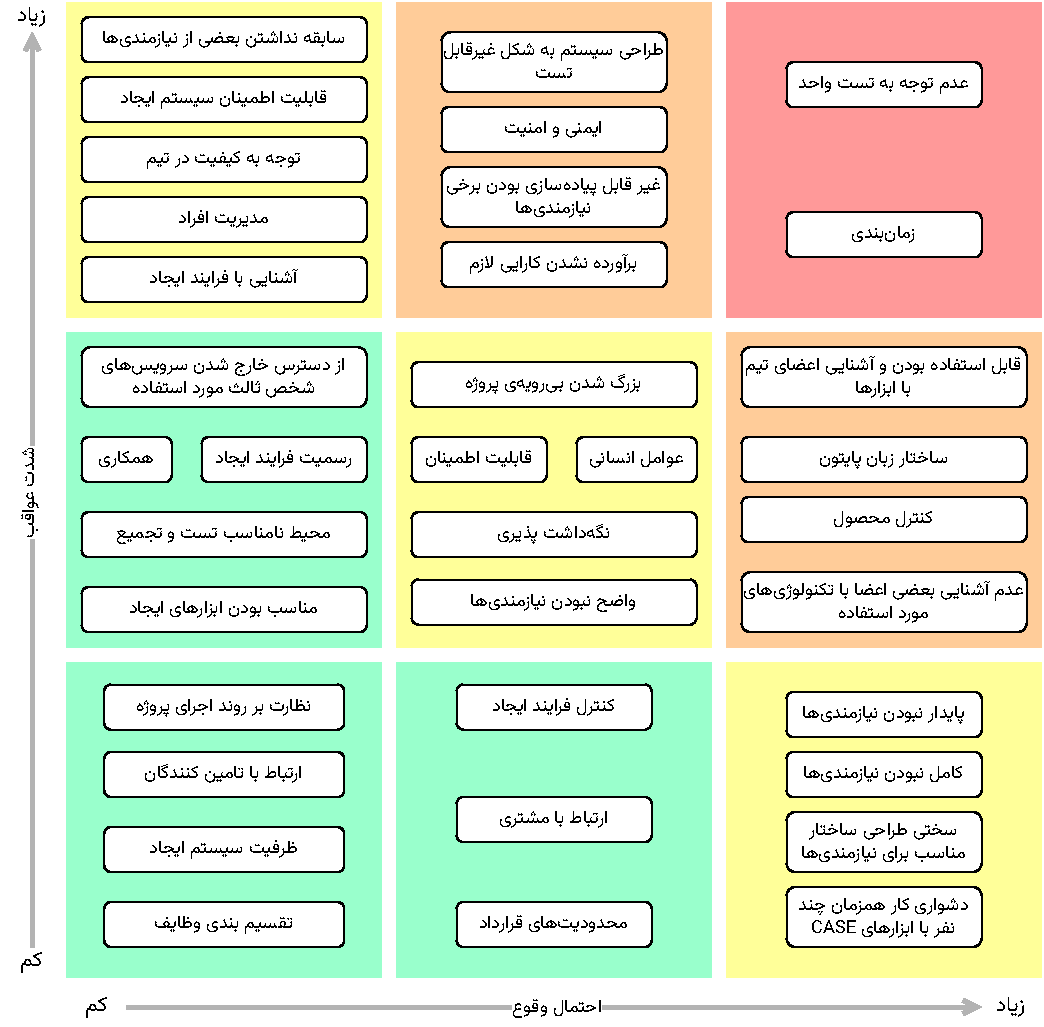
\includegraphics[scale=0.8, page=1]{figs/risks.pdf}
	\caption{اولویت ریسک‌ها}
\end{figure}

